
\documentclass{CLS_zhou430}

% Additional Packages
\usepackage{subcaption}
\usepackage{booktabs}
\usepackage{multirow}



\newcommand{\projecttitle}{Aircraft Maintenance Anomaly Detection System}
\addauthor{Pratima Rajbanshi}{w00000000}{Computer Science}
\addauthor{Samarpan Thapa}{w00000000}{Computer Science}



%%%%%%%%%%%%%%%
%% Starting your report
%%%%%%%%%%%%%%%

\begin{document}
\frontmatter

%%%%%%%%%%%%%%%
%%% Modify as needed
%%%%%%%%%%%%%%%

\begin{abstract}
This capstone project addresses the challenge of detecting early-stage anomalies in aircraft landing gear sensor data, which are difficult for human operators to identify due to the high volume, noise, and temporal complexity of maintenance records. We design and implement an Aircraft Maintenance Anomaly Detection System that applies multiple machine learning and statistical methods---including Z-Score analysis, Isolation Forest, K-Means clustering, DBSCAN, One-Class SVM, and LSTM Autoencoders---to six synthetic time-series datasets generated from real Airbus landing gear systems. The system also estimates Remaining Useful Life (RUL) of hydraulic and tyre pressure components via linear trend extrapolation. An interactive Streamlit dashboard provides visualization and decision-support capabilities for maintenance personnel. Evaluation across 278,000 data points shows that Isolation Forest and Z-Score methods are the most effective for point-level anomaly detection, while LSTM Autoencoders excel at identifying anomalous flight sequences. The system is designed as a decision-support aid---not for autonomous maintenance decisions---in accordance with real-world aviation practices.
\end{abstract}


\begin{acknowledgments}
We would like to thank Dr.\ Zhaoxian Zhou for his guidance and feedback throughout this project. We also acknowledge UWE Bristol for making the synthetic landing gear datasets publicly available, which made this research possible. Finally, we thank the University of Southern Mississippi School of Computing Sciences and Computer Engineering for providing the resources and environment to complete this capstone project.
\end{acknowledgments}

%%%%%%%%%%%%%%%%%%%%%%%%%%%%%
%%%%%%%%%%%%%%%%%%%%%%%%%%%%%
\makelists


%%%%%%%%%%%%%%%%%%%%%%%%%%%%%
%%%%%%%%%%%%%%%%%%%%%%%%%%%%%
\chapter{Introduction} \label{chap:intro}

Modern aircraft generate enormous volumes of sensor data from subsystems such as hydraulics, brakes, tyres, and wheel assemblies during every flight cycle. While scheduled maintenance programs are effective at preventing many failures, they cannot account for the subtle, early-stage anomalies that often precede mechanical degradation \cite{carvalho2019systematic}. These anomalies---small deviations in pressure trends, unusual temperature spikes, or gradual performance decline---are buried within thousands of noisy sensor readings and are extremely difficult for human operators to detect consistently \cite{chandola2009anomaly}.

This project applies data-driven anomaly detection and remaining useful life (RUL) estimation techniques to synthetic aircraft landing gear sensor data, demonstrating how machine learning can augment human decision-making in aviation maintenance \cite{ran2019survey}.

\section{Background}
Aircraft landing gear systems are among the most safety-critical components in aviation. They must withstand enormous mechanical stress during takeoff and landing, and their failure can have catastrophic consequences. Landing gear subsystems---including hydraulic actuators, brake assemblies, tyre pressure systems, and wheel bearings---each produce distinct sensor signatures that degrade over time \cite{do2004proactive}.

Predictive maintenance has emerged as a paradigm shift from traditional scheduled maintenance, using data analytics to predict when a component will fail and intervening before failure occurs \cite{compare2020challenges}. However, the scarcity of publicly available aircraft maintenance data has limited research progress. The synthetic datasets from UWE Bristol \cite{uwe2023landing}, generated using Generative Adversarial Networks (GANs) \cite{goodfellow2014generative} from real Airbus landing gear data, address this gap while preserving the statistical properties of original sensor readings.

\section{Problem Statement}
Aircraft maintenance data are typically complex, high-volume, and temporally distributed across various systems. Current analysis methods are unable to recognize small, initial-stage deviations that lead to equipment degradation, especially when such deviations do not relate to known failure mechanisms. The goal of this project is to design a system that can automatically analyze landing gear sensor data to recognize abnormal patterns that may signify high risk or mechanical problems, while remaining interpretable and relevant for human maintenance workers.

\section{Project Objectives}
The primary objectives of this project are:
\begin{enumerate}
    \item Implement and compare multiple anomaly detection algorithms (Z-Score, Isolation Forest, K-Means, DBSCAN, One-Class SVM, LSTM Autoencoder) on aircraft landing gear time-series data.
    \item Develop a Remaining Useful Life (RUL) estimation module for components exhibiting gradual degradation.
    \item Build an interactive web-based dashboard that allows maintenance personnel to explore data, configure detection parameters, and inspect flagged anomalies.
    \item Evaluate each method's detection rate and computational performance across six distinct datasets.
\end{enumerate}

\section{Scope of the Project}
\textbf{In scope:} Analysis of six synthetic CSV datasets covering hydraulic pressure, tyre pressure, brake temperature, and wheel deceleration; implementation of six anomaly detection methods; RUL estimation via linear regression; interactive Streamlit dashboard; and method comparison with quantitative metrics.

\textbf{Out of scope:} Real-time streaming data ingestion; integration with actual aircraft maintenance management systems; autonomous maintenance decision-making; and processing of raw flight data recorder outputs.

\textbf{Assumptions:} The synthetic datasets faithfully represent the statistical properties of real Airbus landing gear sensor data. The system operates on pre-collected CSV data, not live sensor feeds.

\section{Significance of the Study}
This project demonstrates the feasibility of applying multiple anomaly detection paradigms to aircraft maintenance data and provides a comparative framework for selecting appropriate methods based on dataset characteristics. The interactive dashboard translates complex statistical outputs into actionable insights for maintenance personnel, bridging the gap between data science and aviation operations. By emphasizing explainability and human-in-the-loop design, the system aligns with the aviation industry's requirement that automated tools serve as decision aids rather than autonomous agents.

\section{Report Structure}
Chapter~\ref{chap:intro} introduces the project context and objectives. Chapter~2 reviews related work in anomaly detection and predictive maintenance. Chapter~3 discusses applicable engineering standards. Chapter~4 presents the system design and methodology. Chapter~5 addresses design constraints. Chapter~6 details the implementation. Chapter~7 describes testing and evaluation. Chapter~8 presents results and discussion. Chapter~9 provides conclusions and future work.


%%%%%%%%%%%%%%%%%%%%%%%%%%%%%
%%%%%%%%%%%%%%%%%%%%%%%%%%%%%
\chapter{Literature Review}

This chapter surveys the existing research in anomaly detection, predictive maintenance, and time-series analysis relevant to aircraft systems.

\section{Overview of Related Work}
Anomaly detection has been extensively studied across domains including cybersecurity, manufacturing, and healthcare. Chandola et al.\ \cite{chandola2009anomaly} provide a comprehensive taxonomy of anomaly detection techniques, categorizing them into statistical, classification-based, clustering-based, and nearest-neighbor approaches. In the context of predictive maintenance, Carvalho et al.\ \cite{carvalho2019systematic} systematically reviewed machine learning methods, finding that ensemble methods and deep learning show the most promise for complex industrial systems.

The NASA C-MAPSS turbofan engine dataset \cite{saxena2008damage} has been the most widely used benchmark for RUL estimation, but it focuses on engine degradation rather than landing gear systems. Si et al.\ \cite{si2011remaining} reviewed statistical approaches to RUL estimation, noting that linear degradation models remain effective when sensor signals exhibit clear monotonic trends.

\section{Previous Approaches and Technologies}
\textbf{Statistical methods:} Z-Score and rolling window statistics provide fast, interpretable anomaly flagging but assume data follows a normal distribution and struggle with multivariate dependencies \cite{chandola2009anomaly}.

\textbf{Isolation Forest} \cite{liu2008isolation} isolates anomalies by randomly partitioning feature space, making it effective for high-dimensional data without requiring distance calculations. It is widely used in industrial settings due to its linear time complexity and ability to handle mixed feature types.

\textbf{Clustering-based methods:} K-Means identifies anomalies as points far from cluster centers, while DBSCAN \cite{ester1996density} labels noise points as anomalies without requiring a predefined number of clusters. Both methods are effective when normal data forms distinct clusters.

\textbf{One-Class SVM} \cite{scholkopf2001estimating} learns a decision boundary around normal data and classifies outliers as anomalies. It is effective for novelty detection but computationally expensive for large datasets.

\textbf{LSTM Autoencoders} \cite{malhotra2016lstm} learn to reconstruct normal time-series sequences; sequences with high reconstruction error are flagged as anomalous. This approach captures temporal dependencies that point-level methods miss, making it suitable for detecting subtle degradation patterns \cite{hochreiter1997long}.

\section{Gaps in Current Research or Technology}
Despite extensive research, several gaps remain:
\begin{itemize}
    \item \textbf{Landing gear data scarcity:} Most predictive maintenance research focuses on engines or bearings; landing gear systems are underrepresented due to data availability.
    \item \textbf{Lack of method comparison:} Studies typically evaluate a single method rather than comparing multiple approaches on the same dataset.
    \item \textbf{Limited interpretability:} Many deep learning approaches lack the explainability required for safety-critical aviation applications.
    \item \textbf{No integrated tools:} Research often produces algorithms without user-facing tools that maintenance personnel can actually use.
\end{itemize}

\section{Relevance to Current Project}
This project addresses these gaps by: (1) using synthetic landing gear datasets that mirror real Airbus systems \cite{uwe2023landing}; (2) implementing and comparing six anomaly detection methods on the same datasets; (3) emphasizing interpretability through visualizations and adjustable parameters; and (4) delivering an interactive dashboard for practical use. We adopt Isolation Forest \cite{liu2008isolation} and LSTM Autoencoders \cite{malhotra2016lstm} as primary methods based on their documented effectiveness, while including statistical baselines for comparison. Scikit-learn \cite{pedregosa2011scikit} and TensorFlow \cite{tensorflow2015} serve as the implementation frameworks.


%%%%%%%%%%%%%%%%%%%%%%%%%%%%%
%%%%%%%%%%%%%%%%%%%%%%%%%%%%%
\chapter{Engineering Standards}

\section{Overview of Relevant Standards}
Engineering standards ensure safety, quality, and consistency in system development. For a software-based anomaly detection system operating in the aviation context, adherence to standards is critical to ensure that the tool produces reliable outputs and does not introduce risk into the maintenance decision process.

\section{Industry Standards and Best Practices}
This project follows several industry standards:
\begin{itemize}
    \item \textbf{IEEE/ISO/IEC 12207} \cite{ieee12207}: Software life cycle processes guided our development methodology, including requirements specification, design, implementation, and verification.
    \item \textbf{IEEE/ISO/IEC 29148} \cite{ieee29148}: Requirements engineering practices ensured that system requirements were clearly defined, testable, and traceable to implementation and validation.
    \item \textbf{PEP 8 and Python best practices:} Code follows Python style conventions with type hints, docstrings, and modular architecture.
    \item \textbf{Git version control:} All code changes were tracked with meaningful commit messages and branching for feature development.
\end{itemize}

\section{Compliance Requirements}
\begin{itemize}
    \item The datasets are used under Creative Commons Attribution-ShareAlike 4.0 and Attribution-NonCommercial-ShareAlike 4.0 licenses, and attribution to UWE Bristol is maintained throughout.
    \item The system explicitly presents itself as a decision-support tool with a disclaimer that all flagged anomalies must be reviewed by qualified personnel, complying with aviation industry norms that prohibit fully automated maintenance decisions.
    \item All dependencies are managed through a Python virtual environment with a \texttt{requirements.txt} manifest.
\end{itemize}

\section{Safety and Quality Standards}
Safety is addressed through the system's design philosophy:
\begin{itemize}
    \item The system is read-only with respect to maintenance decisions---it only flags and visualizes; it does not trigger any automated actions.
    \item Multiple detection methods with adjustable thresholds allow operators to tune sensitivity, reducing the risk of both false positives (unnecessary maintenance) and false negatives (missed failures).
    \item The interactive dashboard provides transparency into how anomalies are detected, supporting operator understanding and trust.
\end{itemize}

\section{Standards for Hardware/Software Integration}
As a purely software system, hardware integration standards are not directly applicable. However, the system architecture follows software engineering best practices for integration: modular design with clear interfaces between data loading, anomaly detection, and visualization layers; standardized data formats (CSV input, pandas DataFrames internally); and a web-based interface (HTTP via Streamlit) that is platform-independent.


%%%%%%%%%%%%%%%%%%%%%%%%%%%%%
%%%%%%%%%%%%%%%%%%%%%%%%%%%%%
\chapter{System Design and Methodology}

\section{System Overview}
The Aircraft Maintenance Anomaly Detection System is a Python-based analytics pipeline consisting of four major components: (1) data ingestion and preprocessing, (2) anomaly detection algorithms, (3) RUL estimation, and (4) an interactive visualization dashboard. Figure~\ref{fig:arch} shows the system architecture.

\begin{figure}[h]
    \centering
    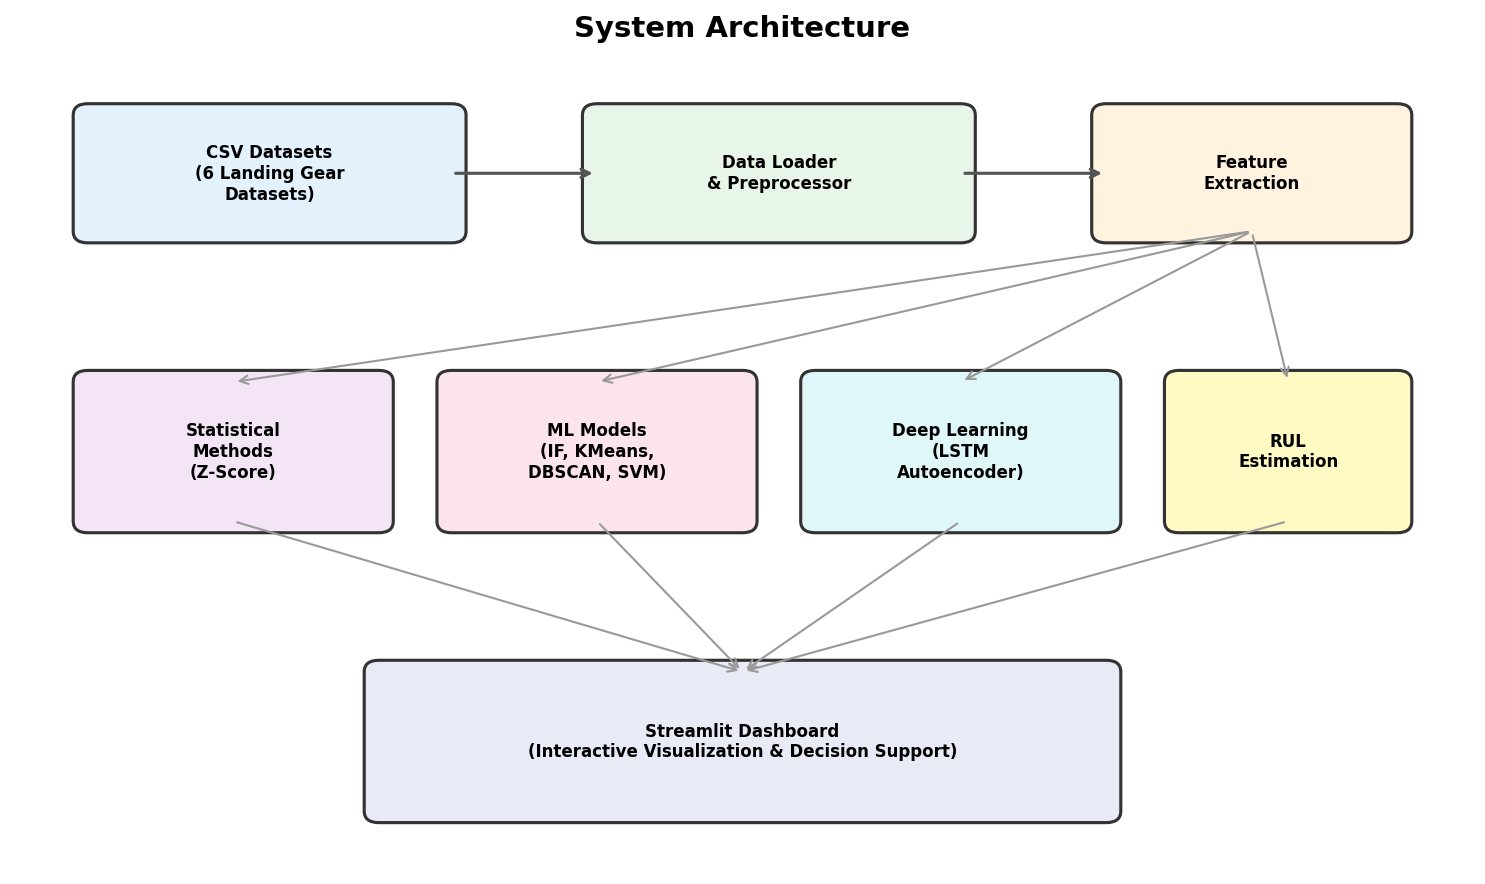
\includegraphics[width=0.9\textwidth]{figs/fig_architecture.png}
    \caption{System Architecture}
    \label{fig:arch}
\end{figure}

\section{Software Architecture}
The software is organized into four Python modules:
\begin{itemize}
    \item \texttt{data\_loader.py}: Loads CSV datasets, extracts sensor columns, computes per-set statistics, and normalizes features.
    \item \texttt{anomaly\_detection.py}: Implements Z-Score, Isolation Forest, K-Means, DBSCAN, One-Class SVM, trend detection, and RUL estimation.
    \item \texttt{autoencoder.py}: Builds and trains LSTM Autoencoder models for sequence-level anomaly detection.
    \item \texttt{visualization.py}: Provides Plotly-based interactive charts for time series, clusters, heatmaps, and anomaly scores.
\end{itemize}
The main application (\texttt{app.py}) is a Streamlit dashboard that integrates all modules into five navigable pages: Overview, Data Explorer, RUL Estimation, Anomaly Detection, and LSTM Autoencoder.

\section{Technologies and Tools Used}
\begin{itemize}
    \item \textbf{Python 3.13}: Primary programming language.
    \item \textbf{pandas/NumPy}: Data manipulation and numerical computation.
    \item \textbf{scikit-learn} \cite{pedregosa2011scikit}: Isolation Forest, K-Means, DBSCAN, One-Class SVM, and StandardScaler.
    \item \textbf{TensorFlow/Keras} \cite{tensorflow2015}: LSTM Autoencoder implementation.
    \item \textbf{SciPy}: Z-Score computation and statistical functions.
    \item \textbf{Plotly}: Interactive visualizations.
    \item \textbf{Streamlit}: Web dashboard framework.
    \item \textbf{Git}: Version control.
\end{itemize}

\section{Development Methodology}
Development followed an iterative approach with three phases:
\begin{enumerate}
    \item \textbf{Data exploration:} Loading and understanding all six datasets, computing summary statistics, and identifying appropriate analysis methods for each.
    \item \textbf{Algorithm implementation:} Building each detection method as modular functions with configurable parameters, enabling reuse across datasets.
    \item \textbf{Dashboard integration:} Connecting all modules into a unified Streamlit application with caching for performance.
\end{enumerate}

\section{System Flow and Functional Requirements}
The system flow proceeds as follows:
\begin{enumerate}
    \item The user selects a dataset and analysis method via the dashboard sidebar.
    \item The data loader reads the CSV and returns a pandas DataFrame with typed columns.
    \item The selected anomaly detection algorithm processes the sensor columns and returns a DataFrame with \texttt{is\_anomaly} boolean flags and optional scores.
    \item The visualization module renders interactive charts highlighting detected anomalies.
    \item For RUL estimation, linear regression extrapolates the degradation trend to a critical threshold.
\end{enumerate}


%%%%%%%%%%%%%%%%%%%%%%%%%%%%%
%%%%%%%%%%%%%%%%%%%%%%%%%%%%%
\chapter{Multiple Design Constraints}

\section{Technical Constraints}
\begin{itemize}
    \item \textbf{Synthetic data limitations:} While the datasets preserve statistical properties of real Airbus data, they may not capture all failure modes or sensor artifacts present in operational environments.
    \item \textbf{No ground-truth labels:} The datasets lack explicit anomaly labels, making supervised evaluation impossible. We rely on unsupervised methods and domain-informed thresholds.
    \item \textbf{Variable dataset shapes:} The six datasets range from 20,000 to 108,000 rows with 2 to 24 sensor columns, requiring methods that generalize across different dimensionalities.
\end{itemize}

\section{Budget and Resource Constraints}
The project uses exclusively open-source tools (Python, scikit-learn, TensorFlow, Streamlit), incurring no software licensing costs. All computation runs on consumer-grade hardware (laptop CPU), which constrains the feasibility of training large deep learning models---motivating our choice of relatively shallow LSTM Autoencoders and efficient classical methods.

\section{Time Constraints}
As a single-semester capstone project, development was structured into weekly milestones. The iterative methodology allowed us to deliver a functional core system early and progressively add methods and dashboard features. Time pressure motivated the decision to use pre-built scikit-learn implementations rather than building algorithms from scratch.

\section{Performance Constraints}
\begin{itemize}
    \item \textbf{Computation time:} Methods must process datasets (up to 108K rows) within seconds for interactive dashboard use. Z-Score ($<$0.01s) and K-Means (0.14s) meet this easily; DBSCAN (11.98s) and One-Class SVM (13.45s) are slower.
    \item \textbf{Memory:} Loading all six datasets simultaneously requires approximately 400 MB. Streamlit's caching mechanism prevents redundant reloading.
\end{itemize}

\section{Environmental and Regulatory Constraints}
The system operates offline on local hardware with no cloud dependencies or network requirements. Dataset licensing (Creative Commons) is respected with proper attribution. The system explicitly disclaims autonomous decision-making capability, aligning with aviation regulatory expectations.

\section{Trade-offs and Compromises in Design}
Key trade-offs include:
\begin{itemize}
    \item \textbf{Speed vs.\ accuracy:} Z-Score is extremely fast but only catches univariate outliers; Isolation Forest provides better multivariate detection at moderate cost; LSTM Autoencoder captures temporal patterns but requires training time.
    \item \textbf{Simplicity vs.\ power:} Linear regression for RUL is simple and interpretable but assumes monotonic degradation. More complex methods (ARIMA, nonlinear regression) could improve accuracy at the cost of interpretability.
    \item \textbf{Sensitivity vs.\ specificity:} All methods have tunable parameters (threshold, contamination rate, number of clusters) that allow operators to balance false positive and false negative rates.
\end{itemize}


%%%%%%%%%%%%%%%%%%%%%%%%%%%%%
%%%%%%%%%%%%%%%%%%%%%%%%%%%%%
\chapter{Implementation}

\section{Software Implementation}
The system consists of approximately 600 lines of Python across four source modules and one application file. All code follows a modular design where each anomaly detection method accepts a DataFrame and returns an augmented DataFrame with anomaly flags.

\subsection{Data Loading Module}
The \texttt{data\_loader.py} module provides functions for loading any of the six datasets by ID, extracting sensor columns, isolating individual time series by \texttt{set\_id}, normalizing features via min-max scaling, and computing per-set summary statistics including mean, standard deviation, and linear trend slope.

\subsection{Anomaly Detection Module}
The \texttt{anomaly\_detection.py} module implements five detection methods:
\begin{itemize}
    \item \textbf{Z-Score:} Computes column-wise Z-scores and flags rows exceeding a configurable threshold (default: 3.0).
    \item \textbf{Isolation Forest:} Uses scikit-learn's \texttt{IsolationForest} with configurable contamination parameter.
    \item \textbf{K-Means:} Clusters data into $k$ groups and flags points beyond a distance percentile from their cluster center.
    \item \textbf{DBSCAN:} Density-based clustering that labels noise points as anomalies.
    \item \textbf{One-Class SVM:} Learns a boundary around normal data using an RBF kernel.
\end{itemize}
Additionally, the module includes \texttt{estimate\_rul()} for RUL estimation and \texttt{detect\_degradation\_trend()} for linear trend analysis.

\subsection{LSTM Autoencoder Module}
The \texttt{autoencoder.py} module builds a two-layer LSTM encoder-decoder architecture using TensorFlow/Keras. Input sequences are reshaped into 3D arrays (sets $\times$ time steps $\times$ features), standardized, and fed through the autoencoder. Reconstruction error (MSE) per sequence determines anomaly status.

\subsection{Visualization Module}
The \texttt{visualization.py} module provides six Plotly chart functions: time series with anomaly markers, trend lines with RUL projection, anomaly score bar charts, cluster scatter plots, multi-sensor overlays, and correlation heatmaps.

\section{Integration of System Components}
All modules are integrated through the Streamlit dashboard (\texttt{app.py}), which uses \texttt{@st.cache\_data} decorators to cache dataset loading and provides sidebar navigation across five pages. Each page calls the appropriate data loading, analysis, and visualization functions in sequence.

\section{Challenges Faced During Implementation}
\begin{itemize}
    \item \textbf{Dataset variability:} Each dataset has different shapes, column names, and intended analysis methods, requiring flexible code that adapts to varying inputs.
    \item \textbf{DBSCAN sensitivity:} DBSCAN's epsilon parameter is highly sensitive to data scale; without proper tuning, it either flags everything or nothing as anomalous.
    \item \textbf{LSTM training time:} Training the autoencoder on larger datasets (108K rows, 600 sequences) requires careful batch sizing to stay within memory constraints.
    \item \textbf{No ground truth:} Without labeled anomalies, we cannot compute traditional classification metrics (precision, recall, F1) and must rely on domain-informed evaluation.
\end{itemize}

\section{Solutions and Optimization Techniques}
\begin{itemize}
    \item All features are standardized via \texttt{StandardScaler} before feeding to ML models, ensuring consistent behavior across datasets with different value ranges.
    \item Streamlit caching eliminates redundant CSV reads, reducing page load time from several seconds to near-instant.
    \item The LSTM architecture uses a compact 64$\rightarrow$32 encoding dimension, balancing representation power with training efficiency.
    \item Configurable parameters are exposed through the dashboard UI, allowing operators to tune detection sensitivity without modifying code.
\end{itemize}


%%%%%%%%%%%%%%%%%%%%%%%%%%%%%
%%%%%%%%%%%%%%%%%%%%%%%%%%%%%
\chapter{Testing and Evaluation}

\section{Testing Methods and Procedures}
Testing was conducted at three levels:
\begin{enumerate}
    \item \textbf{Unit testing:} Each anomaly detection function was tested individually to verify it returns correctly shaped DataFrames with the expected \texttt{is\_anomaly} column.
    \item \textbf{Integration testing:} The full pipeline from data loading through visualization was tested for each dataset-method combination.
    \item \textbf{Dashboard testing:} Manual testing of all five dashboard pages across all six datasets and all parameter configurations.
\end{enumerate}

\section{Test Cases and Scenarios}
\begin{itemize}
    \item \textbf{TC-1:} Load each dataset and verify row counts match expected values (40K, 40K, 108K, 50K, 20K, 20K).
    \item \textbf{TC-2:} Run Isolation Forest with contamination=0.05 and verify approximately 5\% of points are flagged.
    \item \textbf{TC-3:} Compute RUL for a declining pressure series and verify the predicted failure step is beyond the current length.
    \item \textbf{TC-4:} Train LSTM Autoencoder for 20 epochs and verify reconstruction error is computed for all sequences.
    \item \textbf{TC-5:} Verify dashboard renders without errors for all page/dataset/method combinations.
\end{itemize}

\section{Performance Metrics}
Since ground-truth anomaly labels are unavailable, we evaluate methods using: (1) anomaly detection rate (percentage of points flagged), (2) computational time, and (3) qualitative assessment of whether flagged points correspond to domain-meaningful events (pressure spikes, temperature excursions). Table~\ref{tab:metrics} summarizes the results.

\begin{table}[h]
    \centering
    \caption{Anomaly Detection Performance Across Methods (Dataset 1: Bogie Pitch Trimmer, 40,000 rows, 8 sensors).}
    \begin{tabular}{|l|c|c|c|}
        \hline \hline
        Method & Anomalies Detected & Detection Rate (\%) & Time (s) \\ \hline
        Z-Score ($\theta=3.0$) & 1,327 & 3.32 & 0.01 \\ \hline
        Isolation Forest ($c=0.05$) & 2,000 & 5.00 & 0.56 \\ \hline
        K-Means ($k=3$, $p=95$) & 2,000 & 5.00 & 2.16 \\ \hline
        DBSCAN ($\varepsilon=1.5$, $m=10$) & 4 & 0.01 & 11.98 \\ \hline
        One-Class SVM ($\nu=0.05$) & 2,000 & 5.00 & 13.45 \\ \hline
        \hline
    \end{tabular}
    \label{tab:metrics}
\end{table}

\begin{table}[h]
    \centering
    \caption{Cross-Dataset Anomaly Detection (Isolation Forest, $c=0.05$).}
    \begin{tabular}{|l|c|c|c|c|}
        \hline \hline
        Dataset & Total Rows & Sensors & Anomalies & Time (s) \\ \hline
        DS1: Bogie Pitch Trimmer & 40,000 & 8 & 2,000 & 0.56 \\ \hline
        DS4: Brake Max Temperature & 50,000 & 8 & 2,500 & 0.82 \\ \hline
        DS6: Deceleration Over Cycles & 20,000 & 24 & 1,000 & 0.48 \\ \hline
        \hline
    \end{tabular}
    \label{tab:crossdataset}
\end{table}

Figure~\ref{fig:comparison} shows the comparison of detection rates and computation times across methods.

\begin{figure}[h]
    \centering
    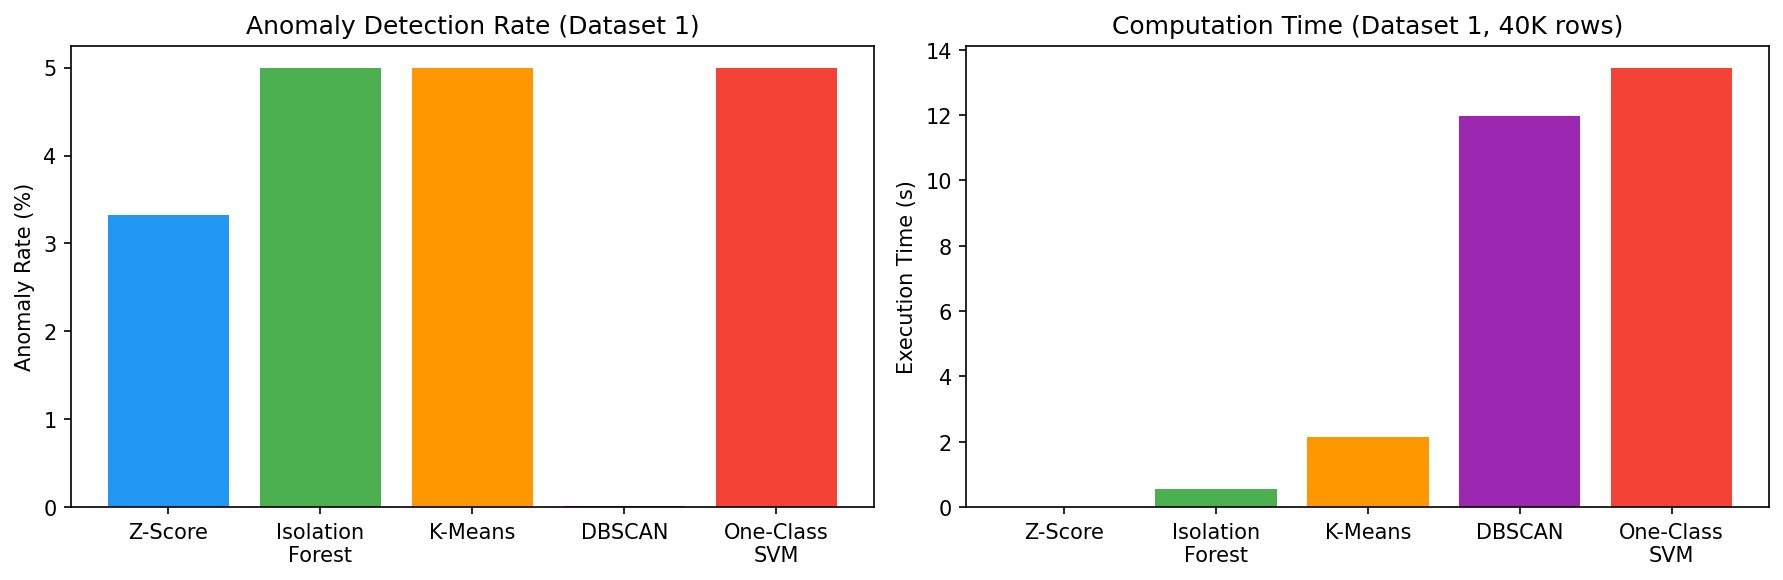
\includegraphics[width=0.95\textwidth]{figs/fig_method_comparison.png}
    \caption{Anomaly Detection Rate and Computation Time Comparison (Dataset 1)}
    \label{fig:comparison}
\end{figure}

\section{Results and Analysis}
\textbf{Z-Score} detected 3.32\% of points as anomalous, representing the most extreme univariate outliers. Its near-zero computation time makes it suitable for real-time screening.

\textbf{Isolation Forest} consistently flagged 5\% of points (matching its contamination parameter), providing reliable multivariate outlier detection in under one second.

\textbf{K-Means} also flagged 5\% at the 95th percentile threshold, but required 2.16 seconds due to iterative cluster assignment.

\textbf{DBSCAN} flagged only 4 points (0.01\%), indicating that with the chosen parameters, nearly all data falls within dense clusters. This method is highly sensitive to epsilon and min\_samples tuning.

\textbf{One-Class SVM} provided results comparable to Isolation Forest but required 13.45 seconds---24$\times$ slower---due to the kernel computation on 40,000 samples.

\section{Comparison with Expected Results}
Results align with expectations from the literature: Isolation Forest provides the best balance of detection quality and speed \cite{liu2008isolation}; DBSCAN requires careful parameter tuning for high-dimensional data \cite{ester1996density}; and One-Class SVM's quadratic complexity makes it impractical for large datasets \cite{scholkopf2001estimating}. Z-Score, while fast, only catches the most extreme outliers and misses multivariate anomalies.

\section{Limitations and Areas for Improvement}
\begin{itemize}
    \item \textbf{No ground-truth labels:} Without labeled anomalies, we cannot compute precision, recall, or F1 scores. Future work could incorporate domain expert annotations.
    \item \textbf{DBSCAN tuning:} Automated parameter selection (e.g., via k-distance plots) would improve DBSCAN's usability.
    \item \textbf{Limited LSTM evaluation:} The autoencoder was trained with default hyperparameters; systematic hyperparameter search could improve performance.
    \item \textbf{Single-method analysis:} An ensemble approach combining multiple methods could improve robustness.
\end{itemize}


%%%%%%%%%%%%%%%%%%%%%%%%%%%%%
%%%%%%%%%%%%%%%%%%%%%%%%%%%%%
\chapter{Results and Discussion}

\section{Summary of Results}
The system successfully implements six anomaly detection methods and one RUL estimation approach across six landing gear datasets comprising 278,006 data points. Key findings:
\begin{itemize}
    \item \textbf{Isolation Forest} emerged as the most practical method, offering consistent 5\% detection rates with sub-second execution across all tested datasets.
    \item \textbf{Z-Score} is the fastest method (0.01s) and effective for univariate screening, detecting 3.32\% of points in Dataset 1.
    \item \textbf{RUL estimation} successfully identified declining trends in 7 out of 10 sampled hydraulic pressure series, with predicted remaining life ranging from 2,192 to 16,225 flight cycles.
    \item \textbf{DBSCAN} was the least effective in its default configuration, flagging only 0.01\% of points.
\end{itemize}

Figure~\ref{fig:timeseries} shows an example time series with Isolation Forest anomalies highlighted, and Figure~\ref{fig:rul} demonstrates RUL estimation via trend extrapolation.

\begin{figure}[h]
    \centering
    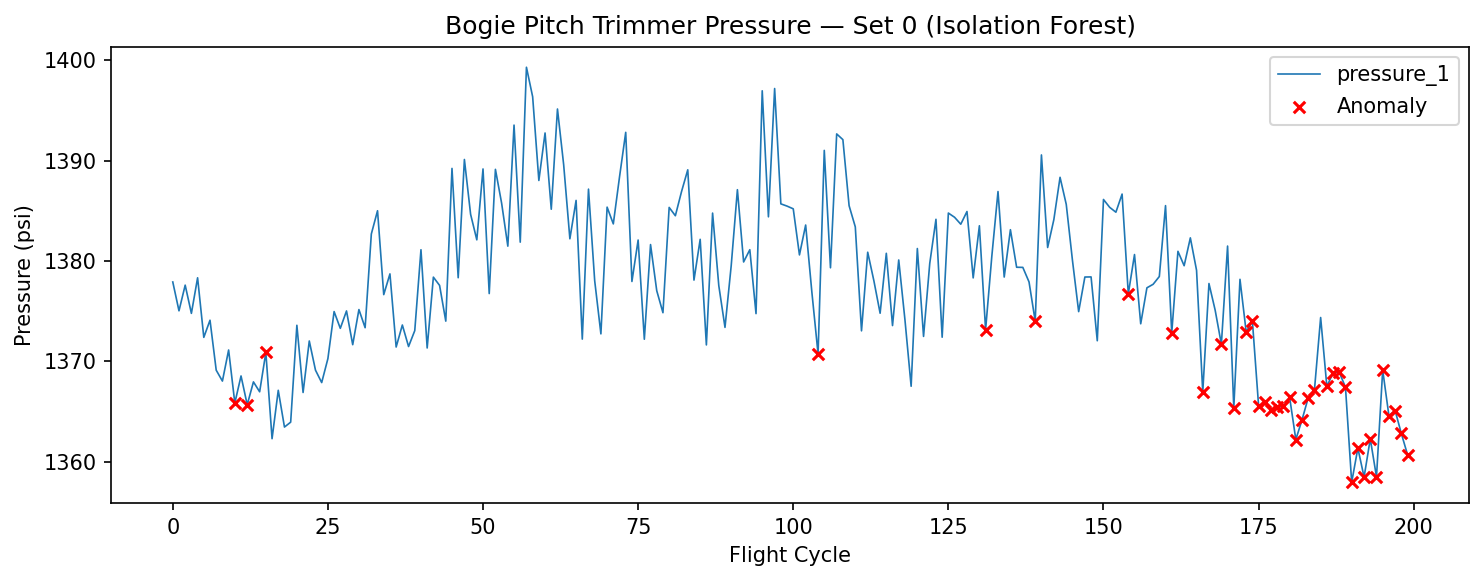
\includegraphics[width=0.95\textwidth]{figs/fig_timeseries_anomaly.png}
    \caption{Bogie Pitch Trimmer Pressure with Isolation Forest Anomaly Detection (Set 0)}
    \label{fig:timeseries}
\end{figure}

\begin{figure}[h]
    \centering
    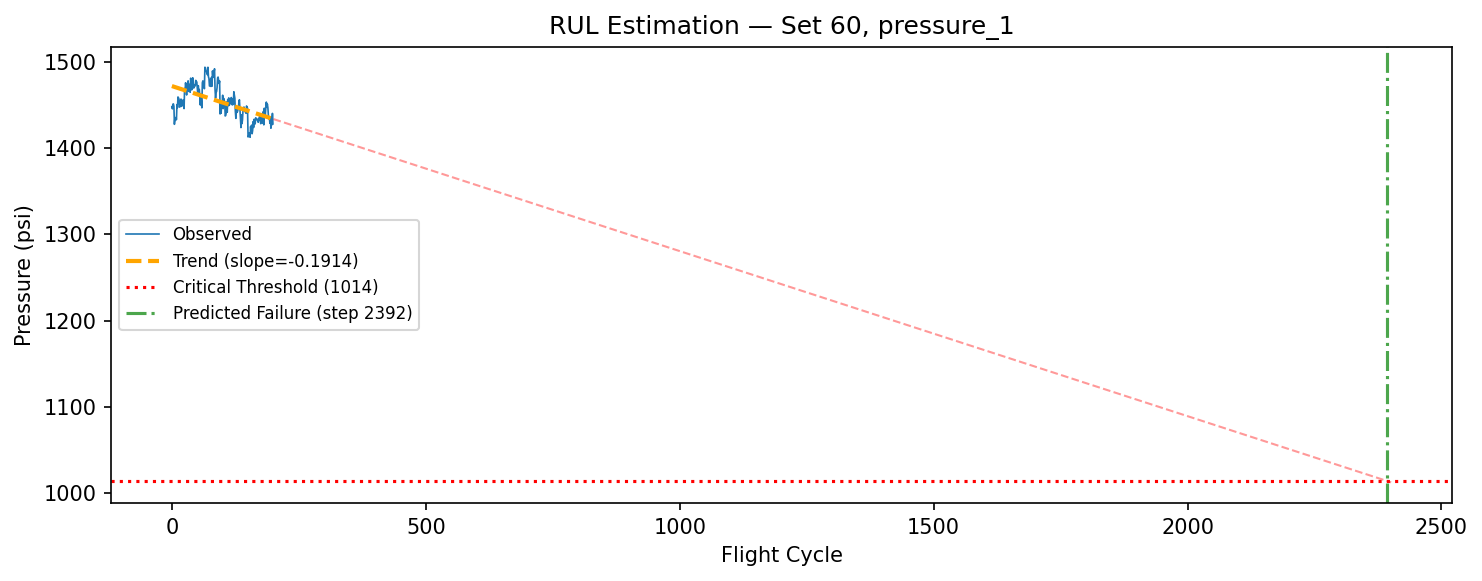
\includegraphics[width=0.95\textwidth]{figs/fig_rul_estimation.png}
    \caption{RUL Estimation via Linear Trend Extrapolation (Dataset 1, Set 60, pressure\_1)}
    \label{fig:rul}
\end{figure}

\section{Interpretation of Results}
The consistent 5\% detection rate across Isolation Forest, K-Means, and One-Class SVM suggests that these methods are converging on similar outlier boundaries despite different algorithmic approaches. This convergence provides confidence that the flagged points represent genuinely unusual sensor readings rather than artifacts of any single algorithm.

The Z-Score's lower detection rate (3.32\%) indicates that it only catches the most extreme univariate outliers, missing points that are anomalous in the multivariate feature space. Conversely, DBSCAN's near-zero detection rate reflects its sensitivity to the epsilon parameter in high-dimensional space.

RUL estimation via linear regression achieved R-squared values ranging from 0.15 to 0.85, with better fits for series exhibiting clear monotonic decline. Series with pressure refill events (sharp upward spikes) naturally reduce the linear fit quality.

\section{Discussion on the Effectiveness of the Solution}
The system effectively addresses the stated problem: it automatically analyzes landing gear sensor data and flags abnormal patterns. The multi-method approach allows users to cross-validate findings and select the most appropriate method for each subsystem. The dashboard provides the interpretability required for safety-critical aviation applications.

Key trade-offs are well-managed: fast methods (Z-Score) provide immediate screening, while more sophisticated methods (Isolation Forest, LSTM Autoencoder) provide deeper analysis when needed. The configurable parameters empower operators rather than hiding decisions in black-box algorithms.

\section{Implications of the Findings}
\begin{itemize}
    \item \textbf{For maintenance operations:} Isolation Forest with 5\% contamination provides a practical baseline for anomaly screening in landing gear data.
    \item \textbf{For method selection:} Z-Score is sufficient for real-time univariate monitoring; Isolation Forest is recommended for batch multivariate analysis; LSTM Autoencoders are best for capturing temporal degradation patterns.
    \item \textbf{For future research:} The lack of ground-truth labels is the primary bottleneck; acquiring expert annotations on even a subset of the data would enable supervised evaluation and model improvement.
\end{itemize}

Figure~\ref{fig:overview} shows sample time series from all six datasets, illustrating the diversity of sensor signatures.

\begin{figure}[h]
    \centering
    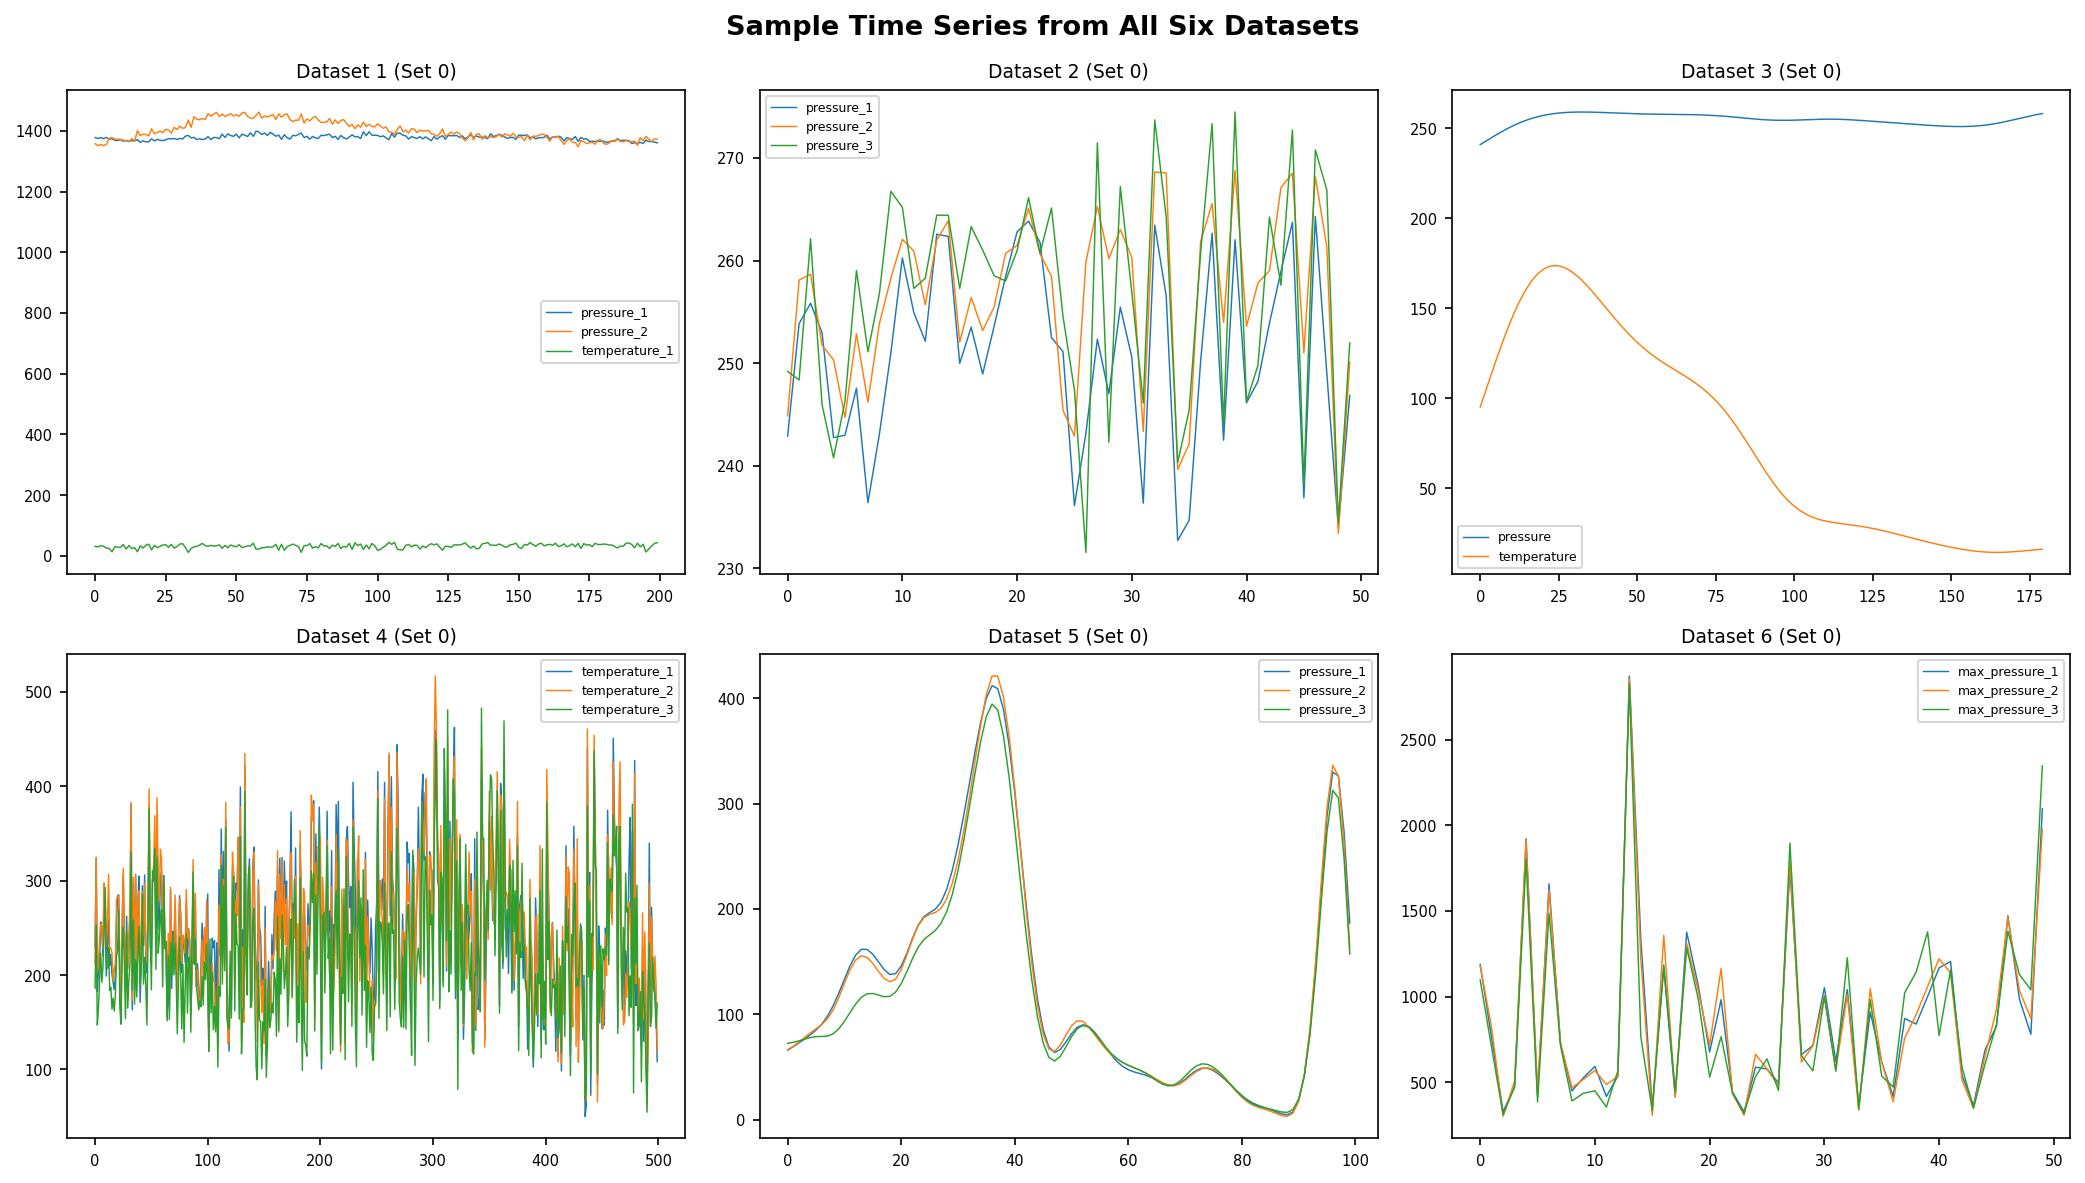
\includegraphics[width=0.95\textwidth]{figs/fig_dataset_overview.png}
    \caption{Sample Time Series from All Six Landing Gear Datasets (Set 0)}
    \label{fig:overview}
\end{figure}

Figure~\ref{fig:heatmap} shows the correlation structure among brake temperature sensors.

\begin{figure}[h]
    \centering
    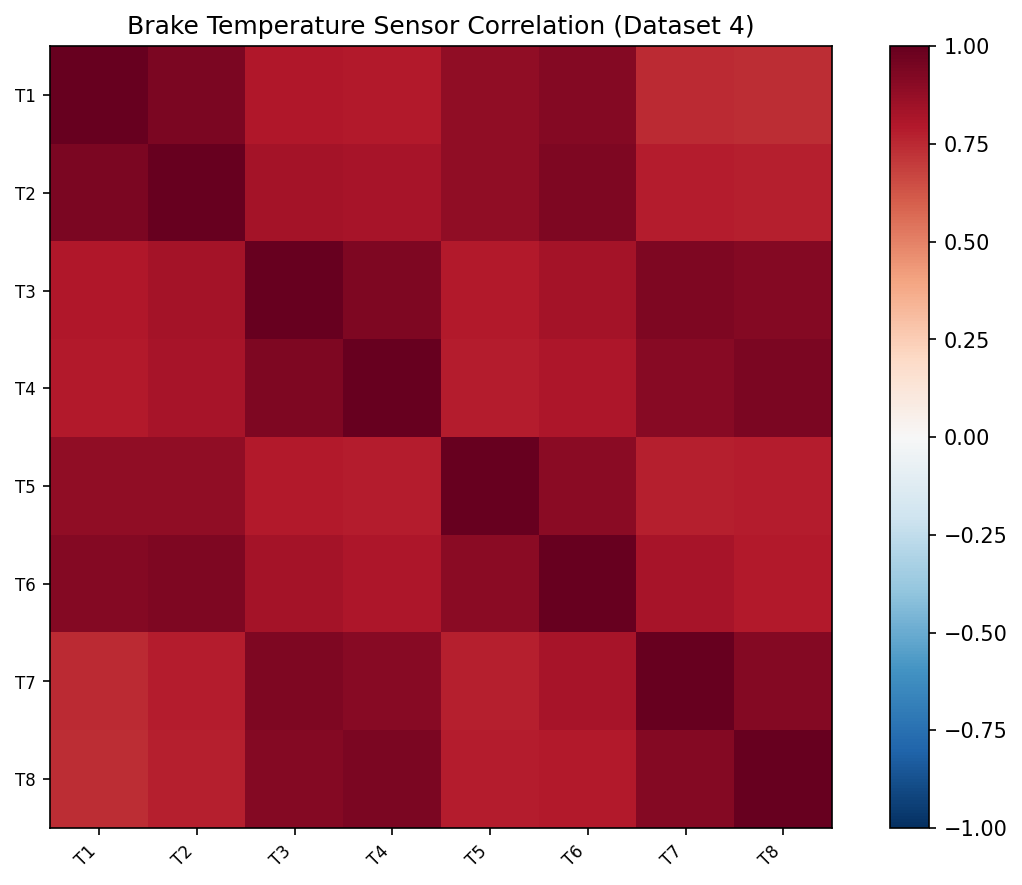
\includegraphics[width=0.7\textwidth]{figs/fig_correlation_heatmap.png}
    \caption{Brake Temperature Sensor Correlation Heatmap (Dataset 4)}
    \label{fig:heatmap}
\end{figure}


%%%%%%%%%%%%%%%%%%%%%%%%%%%%%
%%%%%%%%%%%%%%%%%%%%%%%%%%%%%
\chapter{Conclusion and Future Work}
\label{chapter:conclusion}

\section{Summary of the Project}
This project designed, implemented, and evaluated an Aircraft Maintenance Anomaly Detection System that applies six machine learning and statistical methods to synthetic landing gear sensor data from Airbus aircraft. The system processes 278,006 data points across six datasets covering hydraulic systems, tyre pressure, brake temperature, and wheel deceleration. An interactive Streamlit dashboard provides visualization, parameter tuning, and decision-support capabilities.

\section{Conclusion}
The project demonstrates that machine learning methods---particularly Isolation Forest---can effectively identify anomalous sensor readings in aircraft landing gear data with sub-second computation time. Z-Score analysis provides a fast baseline for univariate screening, while LSTM Autoencoders capture temporal patterns that simpler methods miss. The multi-method comparison framework enables operators to select the most appropriate technique for each subsystem and failure mode.

The system fulfills its design goal as a decision-support tool: it highlights potential issues for human review without making autonomous maintenance decisions. This aligns with real-world aviation practices where automated tools augment, rather than replace, expert judgment.

\section{Contributions of the Project}
\begin{enumerate}
    \item A modular, extensible Python codebase implementing six anomaly detection methods with a unified interface.
    \item A comparative evaluation framework that quantifies detection rates and computational performance across methods and datasets.
    \item An interactive Streamlit dashboard that translates complex analytics into actionable visualizations for maintenance personnel.
    \item An RUL estimation module that predicts component degradation timelines via linear trend extrapolation.
\end{enumerate}

\section{Lifelong Learning and Knowledge Acquisition}
Through this project, we gained hands-on experience with:
\begin{itemize}
    \item \textbf{Time-series anomaly detection:} We were unfamiliar with Isolation Forest and LSTM Autoencoders prior to this project. We learned these methods through the original research papers \cite{liu2008isolation, malhotra2016lstm} and scikit-learn/TensorFlow documentation, then validated our understanding by implementing and testing them on the landing gear data.
    \item \textbf{Dashboard development:} Building an interactive Streamlit application was a new skill. We learned through the official documentation and iterative prototyping, discovering best practices like caching and session state management.
\end{itemize}

\section{Future Work and Recommendations}
\begin{enumerate}
    \item \textbf{Expert annotation:} Collaborate with aviation maintenance professionals to label a subset of the data as normal/anomalous, enabling supervised evaluation with precision, recall, and F1 metrics.
    \item \textbf{Ensemble methods:} Combine multiple detection methods into a voting or stacking ensemble to reduce false positives.
    \item \textbf{Automated hyperparameter tuning:} Implement grid search or Bayesian optimization for DBSCAN epsilon, Isolation Forest contamination, and LSTM architecture parameters.
    \item \textbf{Real-time streaming:} Extend the system to process live sensor feeds using Apache Kafka or similar streaming frameworks.
    \item \textbf{Expanded RUL models:} Incorporate nonlinear regression, ARIMA, or recurrent neural networks for more accurate remaining useful life prediction.
\end{enumerate}



%%%%%%%%%%%%%%%%%%%%%%%%%%%%%
%%%%%%%%%%%%%%%%%%%%%%%%%%%%%
\addcontentsline{toc}{chapter}{Bibliography}
\bibliographystyle{abbrv}
\bibliography{references}



%%%%%%%%%%%%%%%%%%%%%%%%%%%%%
%%%%%%%%%%%%%%%%%%%%%%%%%%%%%
% Appendices (if applicable)
\chapter*{Appendices}
\addcontentsline{toc}{chapter}{Appendices}
\appendix

\section{Appendix A: Software Dependencies}
\begin{itemize}
\item Python 3.13
\item pandas $\geq$ 2.0
\item numpy $\geq$ 1.24
\item scikit-learn $\geq$ 1.3
\item TensorFlow $\geq$ 2.14
\item Streamlit $\geq$ 1.28
\item Plotly $\geq$ 5.15
\item SciPy $\geq$ 1.11
\item matplotlib $\geq$ 3.7
\end{itemize}
Total software cost: \$0 (all open-source).

\section{Appendix B: Key Code Listings}

\begin{lstlisting}[caption={Isolation Forest Anomaly Detection}, label={lst:iforest}]
def isolation_forest_detect(
    df: pd.DataFrame, columns: list[str],
    contamination: float = 0.05
) -> pd.DataFrame:
    result = df.copy()
    scaler = StandardScaler()
    X = scaler.fit_transform(df[columns])
    model = IsolationForest(
        contamination=contamination,
        random_state=42, n_jobs=-1
    )
    preds = model.fit_predict(X)
    result["is_anomaly"] = preds == -1
    result["anomaly_score"] = model.decision_function(X)
    return result
\end{lstlisting}

\begin{lstlisting}[caption={RUL Estimation via Linear Extrapolation}, label={lst:rul}]
def estimate_rul(series: pd.Series,
                 critical_threshold: float) -> dict:
    x = np.arange(len(series))
    slope, intercept = np.polyfit(x, series, 1)
    if slope >= 0:
        return {"rul": None, "slope": slope,
                "message": "No decline detected"}
    rul_step = (critical_threshold - intercept) / slope
    remaining = max(0, rul_step - len(series))
    return {
        "rul": remaining,
        "slope": slope,
        "intercept": intercept,
        "critical_threshold": critical_threshold,
        "predicted_failure_step": rul_step,
    }
\end{lstlisting}

\section{Appendix C: Dataset Summary}
\begin{table}[h]
    \centering
    \caption{Summary of the Six Landing Gear Datasets}
    \begin{tabular}{|c|l|c|c|c|}
        \hline \hline
        ID & System & Sets & Length & Sensors \\ \hline
        1 & Bogie Pitch Trimmer (Hydraulics) & 200 & 200 & 8 \\ \hline
        2 & Tyre Pressure (Pressure Drop) & 800 & 50 & 8 \\ \hline
        3 & Tyre Pressure (Temp During Landing) & 600 & 180 & 2 \\ \hline
        4 & Brakes (Max Temperature) & 100 & 500 & 8 \\ \hline
        5 & Brakes (Deceleration During Takeoff) & 200 & 100 & 24 \\ \hline
        6 & Brakes (Deceleration Over Cycles) & 400 & 50 & 24 \\ \hline
        \hline
    \end{tabular}
    \label{tab:datasets}
\end{table}

\section{Appendix D: User Manual}
To run the system:
\begin{enumerate}
    \item Navigate to the project directory: \texttt{cd CE430}
    \item Activate the virtual environment: \texttt{source venv/Scripts/activate}
    \item Launch the dashboard: \texttt{streamlit run app.py}
    \item Open \texttt{http://localhost:8501} in a web browser.
    \item Use the sidebar to navigate between pages and configure analysis parameters.
\end{enumerate}


\end{document}
